\section{Uncomputing and Recomputing}
\subsection{Tock}
The key insight in zombie is to introduce an abstraction layer on pointers and on the heap, turning pointers, keys into memory space, into tocks, which is 64bit int, keys into logical time.

Tock start at 0, and is increased by 1 on every transition step in the abstract machine, or on every allocation. This created a one-to-one mapping between each transition/lookup(event), with each tock less then the current tock. This had unveil the linear ordering between each events. In particular, a Value allocated during tock X can be recreated by re-executing a transition starting at tock Y < X, because the CEK machine is deterministic, and will replay faithfully what had happened.

Note that for any tock X value, there are, barring edge cases many tock Y < X transition that can replay said value. conversely, for any tock Y, there are multiple tock X > Y value it replay. The one-to-many mapping between transition and values permit us to store asymptotically less metadata than the amount of allocated values.
\subsection{Tock Tree}
To exploit this linearity, the memory space is transformed into a global binary search tree, a Tock Tree, keyed by the tocks.

Each node in the Tock Tree correspond to a state transition. A node at tock t, representing the transition starting at tock t, contain an array of cells(value representations) it allocated, at tock t+1, t+2\dots, paired with the state it transit to. Note that it store the transit-to state, but not the transit-from state, for that state is useless: the transit-from state can recompute the allocated cells during the transition, but we had already stored it anyway!
\begin{figure}
	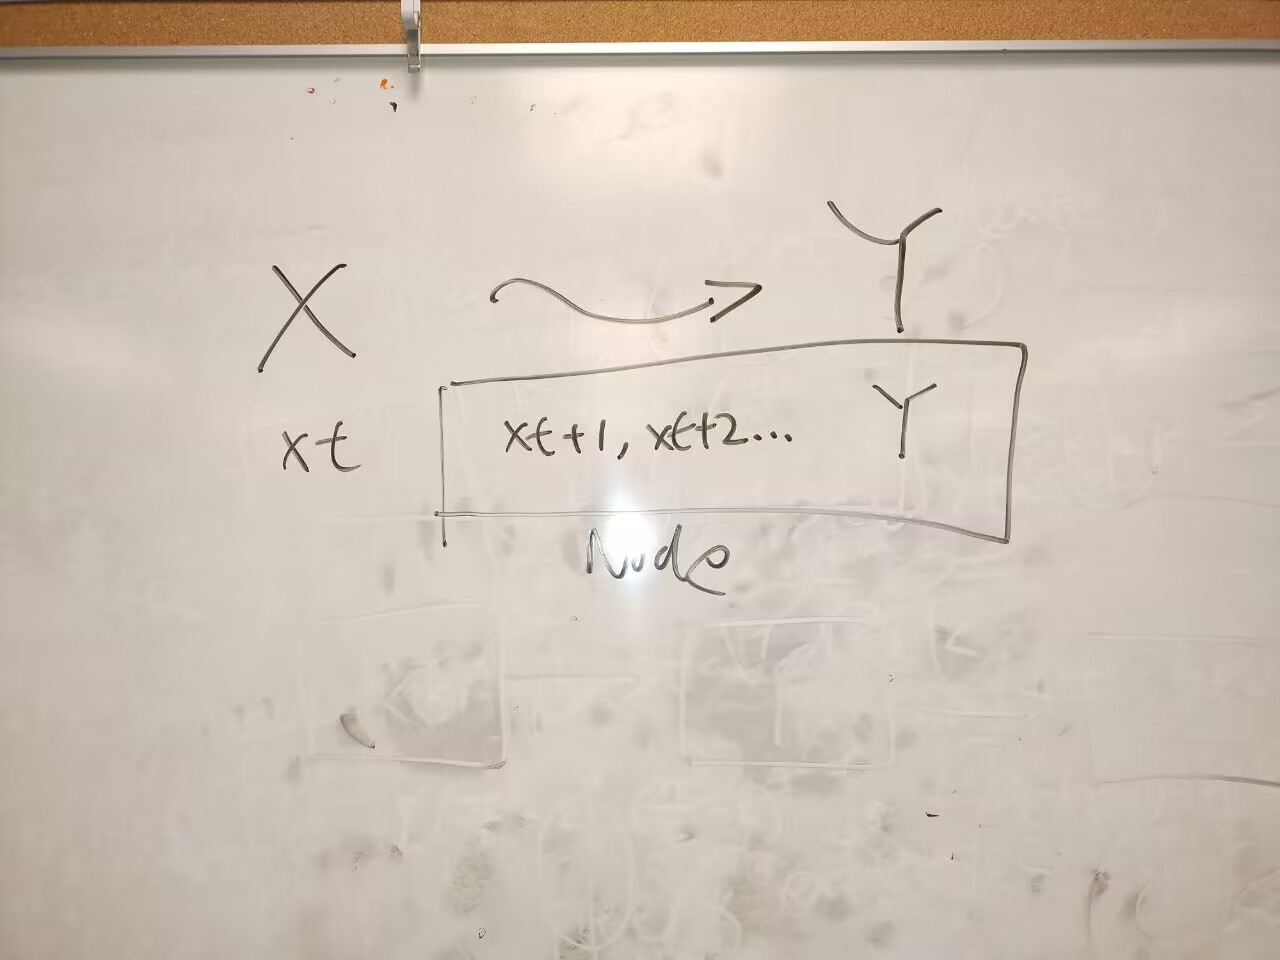
\includegraphics[width=0.5\columnwidth]{2}
	\caption{a node in the tock tree}
\end{figure}
\begin{figure}
	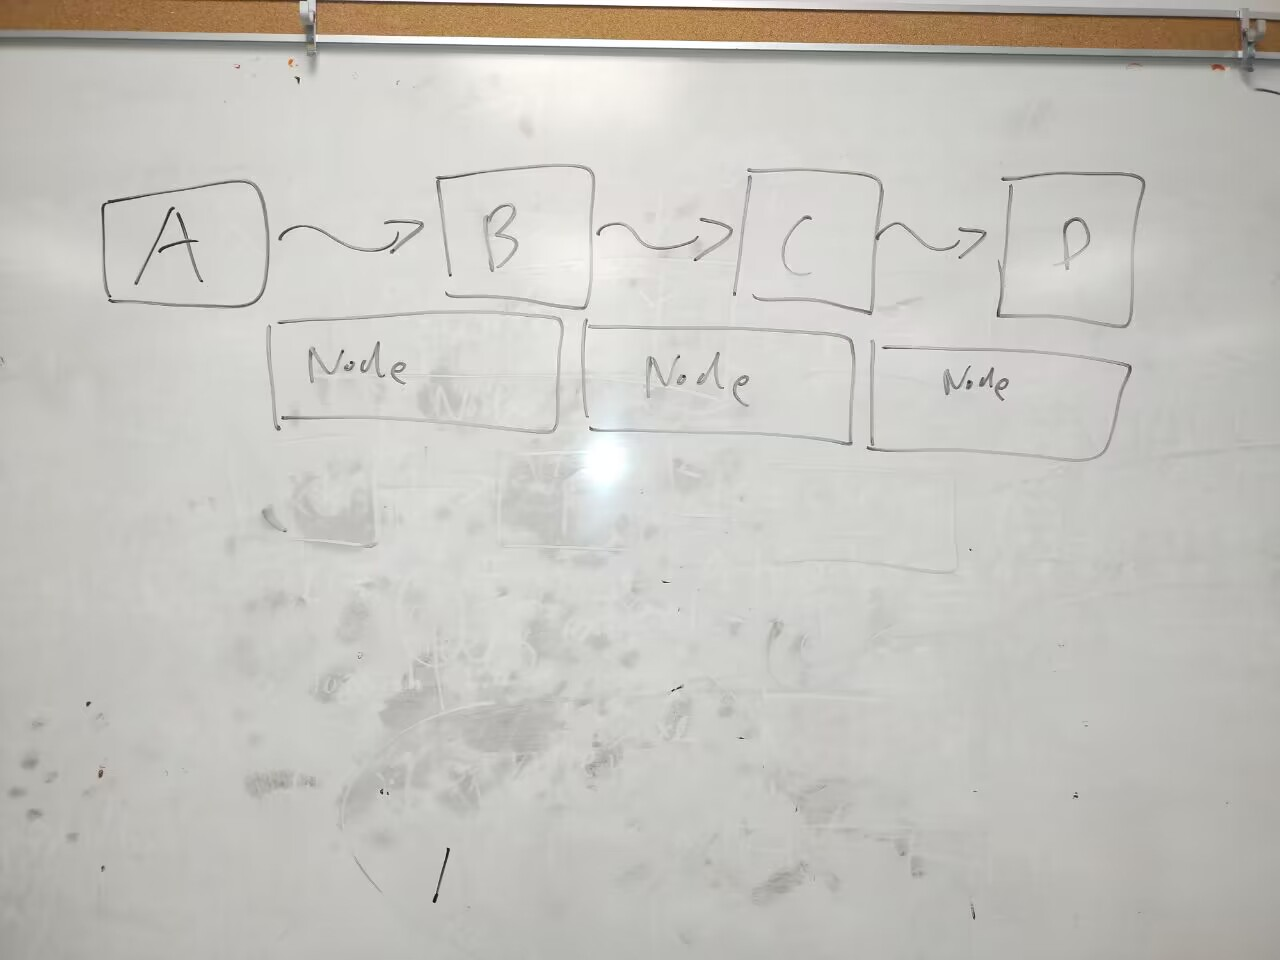
\includegraphics[width=0.5\columnwidth]{3}
	\caption{the tock tree with multiple nodes}
\end{figure}

Unlike binary search tree, which fail when a lookup does not find the precise match, the tock tree is lenient. On a lookup of key x, if said key is not in the tock tree, it will return the node with the largest key y < x instead. Intuitively, this represent returning the latest transition that can replay to the queried node.
\begin{figure}
	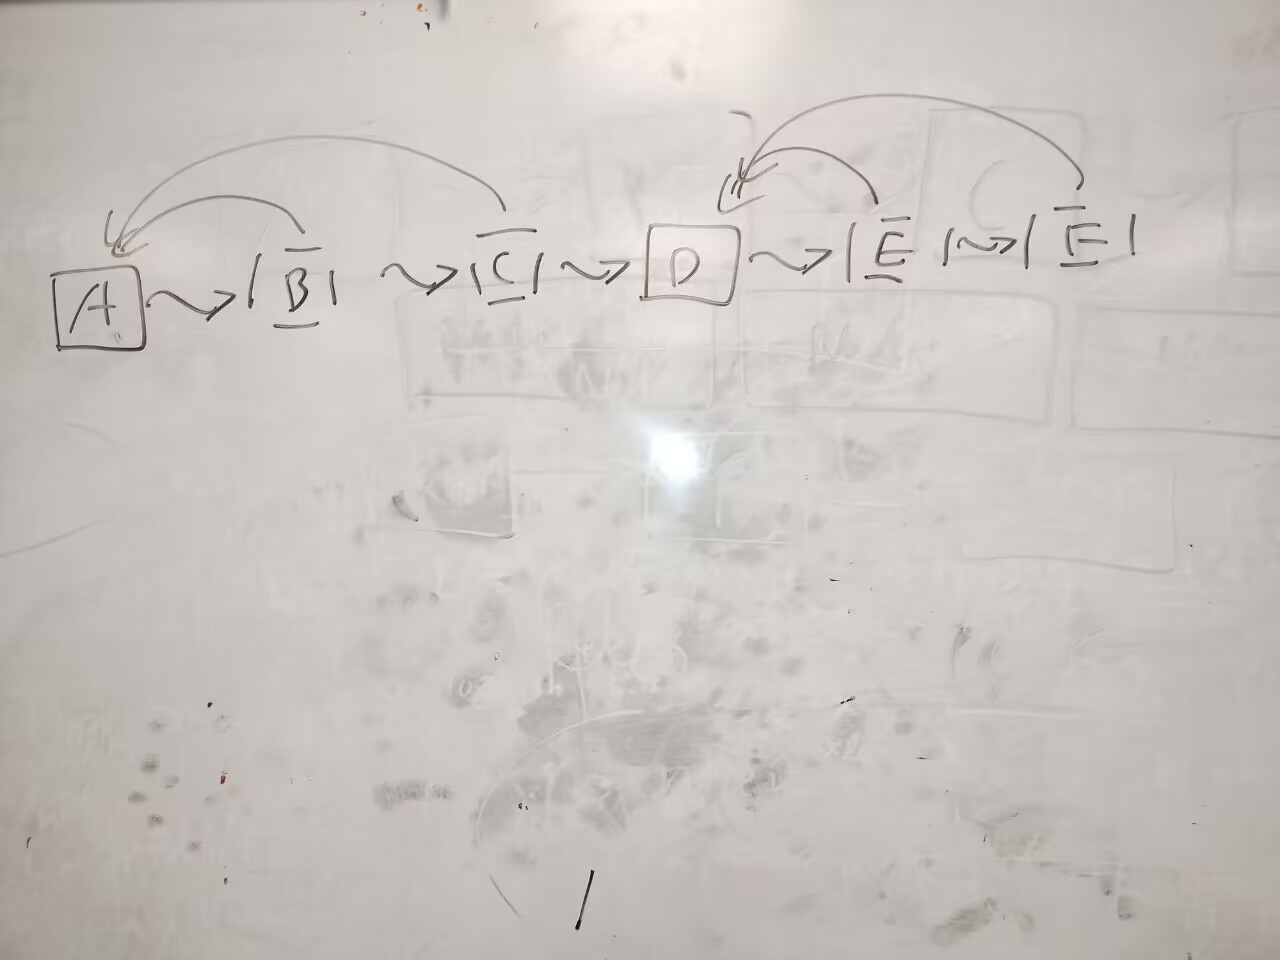
\includegraphics[width=0.5\columnwidth]{4}
	\caption{lookup failure return the latest earlier node}
\end{figure}

This allow us to remove any non-leftmost node from the tock tree. After the removal, the query that originally return the removed node, will return the node slightly earlier then that, which we can then replay to regenerate the removed node. In fact, this is the implementation of uncomputation in our system, and any non-leftmost node can be removed, to save memory at any given time.
\subsection{Happy path}
Every state transition and pointer lookup is then converted into node insertion and node lookup into this data structure. After we had completed a transition, we construct the node, packing the allocated cells during the transition and the transit-to state, inserting the node onto the tock tree.

Originally, transition might require pointers lookup. Such lookup is translated to a query to the tock tree with the given node. Ideally speaking, the returned node contain the cell that correspond to the given tock. We can then convert the tock into the corresponding cell and continue execution. Note that we still need the tock tree to be lenient in this case, as the key of the node denote the beginning of the transition, not the cell itself.
\subsection{Sad Path}
Sadly, as we had removed nodes from the Tock Tree, we might not be able to retrieve a cell directly, and might need to recompute it - the point of the paper.

To recompute a value at tock t, the following steps are taken:
\begin{enumerate}
	\item Suspend the current execution into another kind of continuation, Replay Continuation (RK).
	\item Execute the transit-to state from the lookuped node in the tock tree, until tock reach t.
	\item Resume RK with the cell created at tock t.
\end{enumerate}
Note that the Replay Continuation operate at a more fine-grain granularity then that of the normal continuation. This is because a single transit step might do multiple lookup, but RK need to correspond to a lookup failure in such a transition. Otherwise the requested value might be immediately uncomputed again, and the whole process enter an infinite loop.

After the above 3 steps, the execution shall continue as if no replay had happens at all, and lookup return a node with the cell we wanted. In other words, the happy path and the sad path should converge.

During the replaying process, more lookup might be issued, and those lookup might need more replay - replay is recursive. Just like the classical continuation at the CEK machine, the Replay Continuation need to be recursive, and form a stack as well.

\subsection{Reified Continuation}
We treat continuations also as values, and label them with tock/put them in the tock tree, just like any other values. This allow us to also uncompute continuation as well.